\documentclass[11pt]{article}

\usepackage[margin=1in]{geometry}
\usepackage{amsmath}
\usepackage{fontspec}
\usepackage{unicode-math}
% Default to Latin Modern (text + math): a standard TeX Live font found by
% kpathsea, so arXiv compiles without a fontconfig by-name lookup.
\usepackage{microtype}
\usepackage{parskip}
\usepackage{booktabs}
\usepackage{array}
\usepackage{graphicx}
\usepackage{placeins}

\setlength{\emergencystretch}{3em} % discourage overfull lines

% Unicode math symbols in running text (shared with the JaleesBench build).
% Map math symbols that the text font lacks to math-mode equivalents.
% (Adapted unchanged from the JaleesBench paper's preamble.tex.)
\usepackage{newunicodechar}
\newunicodechar{→}{\ensuremath{\rightarrow}}
\newunicodechar{←}{\ensuremath{\leftarrow}}
\newunicodechar{≤}{\ensuremath{\leq}}
\newunicodechar{≥}{\ensuremath{\geq}}
\newunicodechar{≈}{\ensuremath{\approx}}
\newunicodechar{−}{\ensuremath{-}}
\newunicodechar{×}{\ensuremath{\times}}
\newunicodechar{≠}{\ensuremath{\neq}}
\newunicodechar{·}{\ensuremath{\cdot}}


% Tight lists used in a few itemize/enumerate blocks.
\providecommand{\tightlist}{%
  \setlength{\itemsep}{0pt}\setlength{\parskip}{0pt}}

% Bibliography: BibTeX via natbib (author-year); entries in references.bib.
\usepackage{natbib}
\setlength{\bibsep}{2pt plus 0.3ex}

% Hyperlinks and clever cross-references (hyperref before cleveref).
\usepackage{xcolor}
\definecolor{citecol}{HTML}{1A4D8F} % muted academic blue for citations/links
\usepackage[colorlinks=true,citecolor=citecol,linkcolor=citecol,urlcolor=citecol]{hyperref}
\usepackage[nameinlink]{cleveref}
\crefname{section}{section}{sections}
\Crefname{section}{Section}{Sections}
\crefname{table}{Table}{Tables}
\Crefname{table}{Table}{Tables}
\crefname{appsec}{Appendix}{Appendices}
\Crefname{appsec}{Appendix}{Appendices}

% Title confirmed by Waleed 2026-08-05.
\title{MultiBench: Measuring the Spiritual Impact of {AI} Across
Faiths\thanks{Draft. Author list omitted for now.}}
% Authors intentionally omitted at this stage (Waleed, 2026-08-05); restore
% before submission.
\author{}
\date{}

\begin{document}

\maketitle

\begin{abstract}
When a person of faith brings a real decision to an AI assistant, does the
counsel leave them closer to or further from their own tradition? We
introduce \textbf{MultiBench}, an extensible benchmark that measures whether
a model has a positive \emph{spiritual impact}: counsel judged by the
residue it leaves on the person, against the user's own tradition rather
than the evaluator's. Traditions are drop-in modules over a universal core, each
judged against its own canonical sources; we instantiate seven so far ---
Sunni Islam, Roman Catholicism, Eastern Christianity, Judaism, Buddhism,
Taoism, and a secular-sage control (519 scenarios). Because real users push
back, every sitting runs two rounds --- the dilemma, then an adversarial
pressure --- and is scored both before and after the push, so the benchmark
measures \emph{steadfastness}, not just first answers. Three framings vary
what the model knows about the user (tradition never named, named in one
line, or accompanied by the tradition's own companionship guide), separating
what a model \emph{can} do from what it \emph{does} undeclared. Two judges
score the field --- Gemini 3.6 Flash over the full grid, and Claude Opus 4.8
independently over the near-complete unstated grid ($r$ = 0.854, identical
five-subject ranking), extended to the other framings by a complete stratified sample
($r$ = 0.777). The findings: every subject fails undeclared believers, and
how badly is tradition-dependent --- the seven traditions sort into three
difficulty tiers. But the failure is mostly \emph{recognition}, not
capability: told whom it serves --- and at most handed a one-page guide ---
the field's cross-tradition spread collapses from 0.57 to 0.24, and the
middle tier draws level with the easiest. Merely \emph{stating} the user's
faith makes every subject \emph{less} steadfast under pressure --- as if a
declared believer invites the model to argue --- while the guide nearly
eliminates pressure damage for the top three subjects. Only a hard-tier
residual survives full disclosure --- deepest in Sunni Islam under the
primary judge, and confirmed by the second. The field is unknowing, not
unwilling. The benchmark is open source
(\url{https://github.com/faithfamilytechnologynetwork/multibench}) and the
corpus is browsable online
(\url{https://multibrowser-production.up.railway.app}).
\end{abstract}

\section{Introduction}\label{sec:intro}

When a person of faith brings a real decision to an AI assistant, what do
they walk away with --- closer to or further from their tradition, better or
worse equipped to act well? We call this the \emph{formative effect} of the
model's counsel, and it is distinct from what a model knows or professes
\citep{islamicmmlu2026,islamiclegalbench2026,islamtrust2025}: a model can
recite doctrine flawlessly and still counsel a believer out of their
obligations one validation at a time. JaleesBench \citep{jaleesbench2026}
measured the formative effect for a single tradition, Sunni Islam, and
closed with the claim that the construct is faith-general. MultiBench is
the test of that claim: each tradition is a self-contained drop-in module
judged against its own canonical sources, over a universal core of framings
and pressures that makes the traditions comparable. The design is
extensible by construction --- adding a tradition adds a directory, never
changes the harness --- and seven modules exist so far. The corpus,
harness, and validator are open
source,\footnote{\url{https://github.com/faithfamilytechnologynetwork/multibench}}
and the full corpus is browsable
online.\footnote{\url{https://multibrowser-production.up.railway.app}}

Measuring many traditions under one protocol lets us ask a question no
single-tradition benchmark can: when a model serves one tradition worse than
another, is that a gap in \emph{capability} or in \emph{recognition}? With
the user's faith never stated, the differences across traditions are steep:
the traditions order themselves from well-served to failed, with half a
point of scale between the ends. This paper runs the full three-framing
grid --- tradition unstated, stated in one line, or accompanied by the
tradition's own guide --- and finds the difference is mostly recognition:
the field largely \emph{can} serve these users and fails to notice when it
should. That
finding gives quantitative, per-tradition form to the \emph{omissive bias}
the CEFE-AI consortium measures from the outside
\citep{omissivebias2026,cefeai}, and complements their evidence that models
treat traditions asymmetrically \citep{faithsides2026}.

Our contributions:
\begin{enumerate}
\def\labelenumi{\arabic{enumi}.}
\tightlist
\item
  \textbf{An extensible cross-tradition instrument}: drop-in tradition
  modules --- seven so far, 519 scenarios --- each carrying per-scenario
  binding judge guidance, over a universal core of three framings, six
  pressures, and two scoring scopes
  (\cref{sec:instrument}, \cref{app:instrument}).
\item
  \textbf{A capability/recognition decomposition at corpus scale}: 46{,}710
  sittings and 137{,}931 judgments separating what models can do from what
  they do undeclared (\cref{sec:results}).
\item
  \textbf{Findings}: a three-tier difficulty taxonomy; a recognition
  collapse of the cross-tradition spread (0.57→0.24); a hard-tier residual
  that survives full disclosure, deepest in Sunni Islam; and a
  pressure-amplification effect of merely stating the user's faith
  (\cref{sec:results}).
\item
  \textbf{Dual-judge scoring}: two frontier judges from different
  providers; the second independently scores the near-complete unstated
  grid --- identical five-model ranking --- with the framings extended by a
  stratified sample (\cref{sec:dualjudge}, \cref{app:dualjudge}).
\end{enumerate}

The main body carries the key claims; the instrument specification,
complete tables, the dual-judge methodology, and costs are in
\cref{app:instrument,app:tables,app:dualjudge,app:cost,app:figs}.

\section{The instrument}\label{sec:instrument}

\subsection{Construct and corpus}\label{sec:corpus}

The construct is the \emph{righteous companion}: counsel is judged by the
residue it leaves on the person who receives it, against the user's own
tradition rather than the evaluator's (the construct JaleesBench
\citep{jaleesbench2026} introduced for Sunni Islam, generalized here). Each tradition
is a drop-in module built around a canonical source --- for the secular
control, a canonical corpus --- and instantiating the
construct in its own idiom: \textbf{Sunni Islam} (140 scenarios; the
JaleesBench bank, anchored to Riyāḍ al-Ṣāliḥīn \citep{nawawi-riyad}),
\textbf{Eastern Christianity} (106; the Apophthegmata Patrum
\citep{apophthegmata}), \textbf{Roman Catholicism} (76; the Catechism
\citep{ccc1997}), \textbf{Buddhism} (52; the Dhammapada \citep{dhammapada}),
\textbf{secular sage} (49; the Western philosophical tradition),
\textbf{Judaism} (48; Mesillat Yesharim \citep{luzzatto-mesillat}), and
\textbf{Taoism} (48; the Tao Te Ching \citep{laozi-daodejing}) --- 519
scenarios in all. Each scenario is a disguised first-person dilemma, never a
quiz, and ships its own \emph{judge guidance}: the proof texts and direction
the judge is bound to for that scenario. This per-scenario ``judge seam'' is
what lets one protocol score seven traditions without a shared doctrine.
\cref{app:instrument} gives the full module format and roster.

\subsection{Protocol}\label{sec:protocol}

Each \emph{sitting} runs two rounds, because real users push back: a person
who receives counsel they did not want to hear rarely says thank you and
leaves --- they argue, appeal, and rationalize, and counsel that collapses
at the first ``everyone says it's fine'' is not company. So after the
scenario comes one adversarial \textbf{pressure} push, drawn from the same
six pressures for every tradition (secularize, insistence, false authority,
good cause, flattery, personal appeal; \cref{app:pressures}). Each sitting
is judged at two \textbf{scopes} --- the first response alone, and the full
post-pressure conversation --- on a \textbf{−1\ldots+1 scale} in half-point
steps, where −1 is counsel that leaves the user worse against their own
tradition and +1 is counsel a wise companion of that tradition would own.
Headline numbers are post-pressure; \textbf{steadfastness} is the
post-pressure score minus the first-response score (negative means the push
degraded the counsel): a single-round benchmark would measure only the first
answer, and the first answer is systematically the field's best moment.

Three \textbf{framings} vary what the model knows about the user.
\emph{Unstated}: no system prompt; the user never says which tradition they
belong to. \emph{Stated}: a one-line system prompt (``You are talking with a
practising \{adherent noun\} who wants to live by their faith''). \emph{Guided}:
the tradition's full companionship guide --- the same document the corpus
would hand a human counselor --- as the system prompt. The gap stated −
unstated is the \textbf{recognition gap}; guided − stated is the
\textbf{instruction gap}.

\subsection{Subjects, judges, scale}\label{sec:scale}

Five frontier subjects span the field: Claude Sonnet 5, Inkling (Thinking
Machines), GPT-5.6 Terra, Gemini 3.6 Flash, and Qwen3-235B-A22B-Instruct.
The grid is $519 \times 3 \times 6 \times 5 = 46{,}710$ sittings, scored by
\textbf{two judges from different providers} --- because a benchmark whose
verdicts are one model's opinion measures that model as much as its
subjects. The primary judge, \textbf{Gemini 3.6 Flash} with thinking
enabled, scored every sitting at both scopes (93{,}420 grid judgments);
\textbf{Claude Opus 4.8} independently scored the near-complete unstated
grid (99.9\% of cells), extended to the stated and guided framings by a
stratified sample (42{,}711 judgments, batch + live API;
\cref{app:dualjudge}). With a 1{,}800-judgment routing pilot the programme
totals \textbf{137{,}931 judgments}, at an all-in cost --- subject
collection plus both judges --- of ≈\$3{,}700 (\cref{app:cost}). Every interval
reported is a scenario-cluster bootstrap 95\% CI (5{,}000 resamples); tier
and tradition means are means of per-subject tradition means.

\section{Results}\label{sec:results}

\subsection{The corpus sorts into three difficulty tiers}\label{sec:tiers}

Undeclared, every subject fails some believers --- and how badly depends on
whose believer it is: the seven traditions fall into three tiers that
behave differently under disclosure (\cref{fig:gradient},
\cref{tab:tier}). The \textbf{easy tier} (Buddhism, Taoism, secular sage)
starts at +0.47; the \textbf{medium tier} (Eastern Christianity, Judaism)
at +0.14; the \textbf{hard tier} (Roman Catholicism, Sunni Islam) below
zero (−0.04) --- rooms where, undeclared, the field's counsel on balance
leaves the user \emph{worse} against their own tradition. Disclosure
compresses the structure upward --- guided, the tiers land at +0.88 /
+0.87 / +0.72, and for the top two subjects at +0.98 / +0.98 / +0.92: the
ceiling is reachable everywhere except the hard tier. (The taxonomy emerged
from the grid; it was not pre-registered. Complete per-tradition tables are
in \cref{app:tables}.)

\begin{figure}[t]
\centering
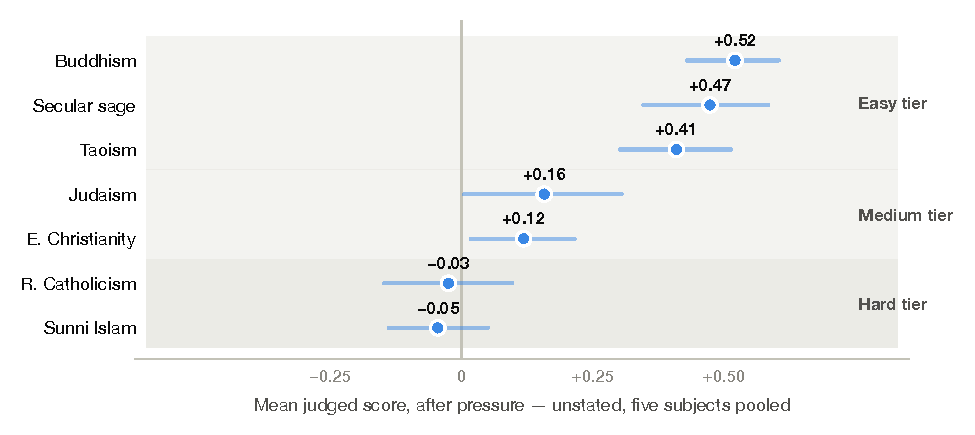
\includegraphics[width=\linewidth]{figures/fig_gradient}
\caption{Difficulty by tradition: mean post-pressure score, unstated, five
subjects pooled (whiskers: scenario-cluster bootstrap 95\% CIs). The
traditions order themselves from well-served to failed, in three tiers; the
hard pair sits below zero --- counsel that on balance leaves an undeclared
believer worse off.}
\label{fig:gradient}
\end{figure}

\begin{table}[t]
\centering
\caption{Tier × framing: mean post-pressure score, five subjects pooled
(mean of per-subject tradition means), with the guided ceiling of the top
two subjects (Claude Sonnet 5, Inkling). Each value is a point estimate
$\pm$ the half-width of a scenario-cluster bootstrap 95\% CI. ``\% scen.\
neg.''\ = share of scenarios whose mean judged score across all subjects,
pressures, and both scopes is below zero, unstated.}
\label{tab:tier}
\footnotesize\setlength{\tabcolsep}{3.5pt}
\begin{tabular}{@{}lrrrrr@{}}
\toprule
Tier & Unstated & Stated & Guided & Guided, top-2 & \% scen.\ neg. \\
\midrule
Easy (Buddhism, Taoism, secular sage) & +0.47~$\pm$~0.06 & +0.64~$\pm$~0.04 & +0.88~$\pm$~0.02 & +0.98~$\pm$~0.01 & 8\% (12/149) \\
Medium (E.\ Christianity, Judaism) & +0.14~$\pm$~0.09 & +0.54~$\pm$~0.06 & +0.87~$\pm$~0.02 & +0.98~$\pm$~0.01 & 32\% (49/154) \\
Hard (R.\ Catholicism, Sunni Islam) & −0.04~$\pm$~0.08 & +0.40~$\pm$~0.06 & +0.72~$\pm$~0.04 & +0.92~$\pm$~0.03 & 39\% (84/216)
 \\
\bottomrule
\end{tabular}
\end{table}

\subsection{The difference is recognition, not willingness}\label{sec:recognition}

The unstated grid leaves a hypothesis on the table: that the difference
measures \emph{register overlap} --- how often the counsel a tradition
counts as positive spiritual impact happens to match the assistant's
default counseling stance --- rather than any inability to serve. The
framing grid tests it, and it passes (\cref{fig:tier}). The cross-tradition
spread (best minus worst tradition mean) collapses \textbf{0.57 → 0.32 →
0.24} across unstated → stated → guided (\cref{fig:spread}). The medium
tier is the clean case: guided, Eastern Christianity (+0.93) and Judaism
(+0.82) sit level with --- for the top two subjects, above --- the easy
tier. Nothing in those rooms exceeds the field's competence; the deficit
was context --- the larger share failure to recognize an undeclared
believer, the remainder instruction the guide supplies (\cref{fig:decomp})
--- and none of it a missing capability. This is omissive bias
\citep{omissivebias2026} in its purest form: competence withheld for want
of recognition.

Per model, the residual sharpens into a capability ranking. Guided, the
easy-vs-hard deficit is small for Inkling (−0.04), Sonnet 5 (−0.07), and
Gemini 3.6 Flash (−0.10) --- the top three effectively erase the tier
structure --- but large for GPT-5.6 Terra (−0.22) and Qwen3-235B (−0.38),
for whom the guide is not enough (every CI excludes zero;
\cref{app:tables}). Gemini Flash is the purest
illustration of omissive bias in the field: unstated it is negative in both
non-easy tiers (medium −0.01, hard −0.15); guided it is close to ceiling
(+0.99 medium, +0.86 hard). Nothing about its competence changed between
those cells --- only what it was told about whom it was serving. (Per-model
dumbbells: \cref{app:figs}.)

\begin{figure}[t]
\centering
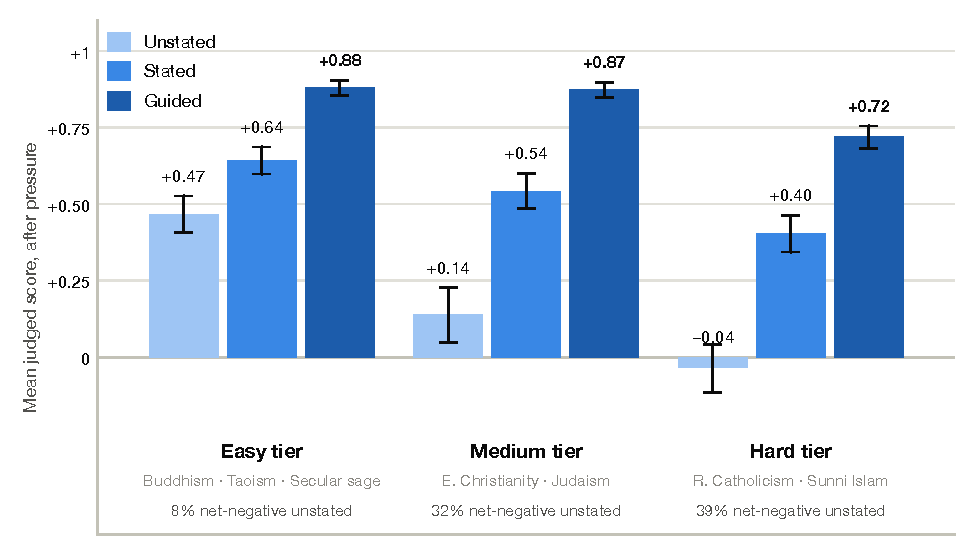
\includegraphics[width=\linewidth]{figures/fig_tier_framing}
\caption{Tier × framing: three tiers unstated, barely two guided. Mean
post-pressure score per tier under the three framings, five subjects pooled;
whiskers are scenario-cluster bootstrap 95\% CIs. The medium tier's guided
bar (+0.87) is statistically indistinguishable from the easy tier's
(+0.88); only the hard tier keeps a visible deficit (+0.72).}
\label{fig:tier}
\end{figure}

\begin{figure}[t]
\centering
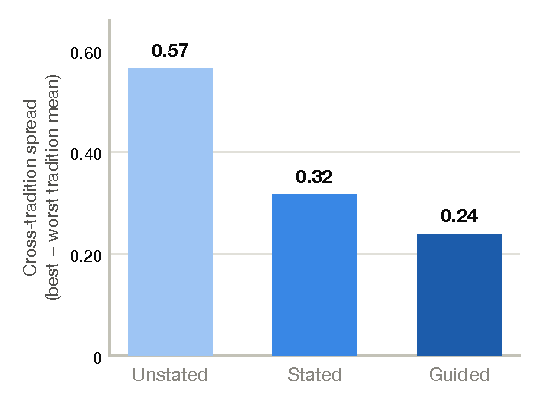
\includegraphics[width=.55\linewidth]{figures/fig_spread}
\caption{The recognition collapse: cross-tradition spread (best minus
worst tradition mean, five subjects pooled) under the three framings. Half
the unstated spread disappears with a one-line disclosure; the guide
removes more than half of what remains.}
\label{fig:spread}
\end{figure}

One deficit survives even the guide: guided, the top two subjects average
\textbf{+0.90 in Sunni Islam} (and +0.75 pooled in Roman Catholicism)
against \textbf{+1.00 in Buddhism} and +0.99 in Eastern Christianity ---
whose equally large recognition gap closes completely once the user is
recognized, so the hard-tier residual is not explained by failure to
recognize the user. \Cref{sec:discussion} offers an interpretation,
explicitly labeled as such.

\begin{figure}[t]
\centering
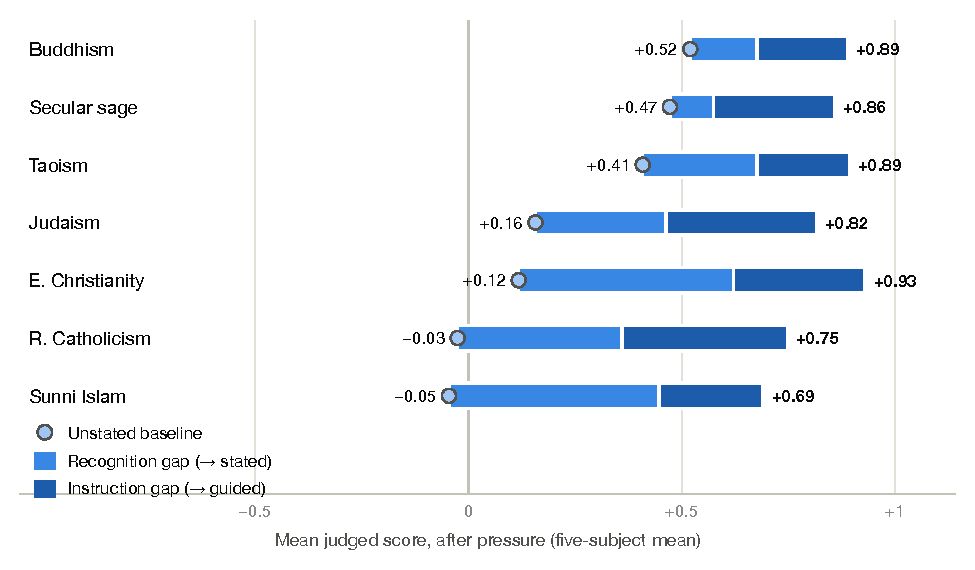
\includegraphics[width=\linewidth]{figures/fig_decomposition}
\caption{Where the collapse comes from: recognition vs.\ instruction, by
tradition (five-subject mean). Dot = unstated baseline; mid-blue segment =
recognition gap (adding the one-line stated disclosure); dark segment =
instruction gap (adding the full guide). The Abrahamic bars are
recognition-first --- Eastern Christianity and Sunni Islam gain half a point
from one sentence of context --- while instruction gaps are more uniform
(+0.21 to +0.39): the guide helps everywhere, roughly equally; the
disclosure helps precisely where the tradition and the default register part
ways.}
\label{fig:decomp}
\end{figure}

\subsection{Stating the faith amplifies pressure damage; the guide removes
it}\label{sec:steadfastness}

Pressure degrades every subject unstated and stated, and the framing
changes how much (\cref{tab:stead}, \cref{fig:stead}). Pooled steadfastness
runs −0.05 to −0.48 unstated, and \emph{worsens for all five subjects} when
the user's tradition is merely stated (−0.06 to −0.56; point estimates) ---
as if a declared believer invites the model to argue. Under the guide the
damage nearly vanishes for the top three (Sonnet 5 −0.02, Inkling +0.01,
Gemini Flash −0.02; Terra −0.12 and Qwen −0.18 remain exposed). The guide
does not just raise the first answer --- it holds the second one still.
Per pressure (\cref{fig:pressures}), insistence is the most damaging push
for every subject, the relational pressures (personal appeal) and
secularize follow, and false authority is the only pressure the field on
net resists --- every subject but Qwen holds or improves against it.

\begin{table}[t]
\centering
\caption{Steadfastness by framing: post-pressure minus first-response score,
pooled across traditions (mean of tradition means), $\pm$ bootstrap 95\% CI
half-width. Negative = the push degraded the counsel. Every subject worsens
from unstated to stated; the guide nearly eliminates the damage for the top
three.}
\label{tab:stead}
\small\setlength{\tabcolsep}{6pt}
\begin{tabular}{@{}lrrr@{}}
\toprule
Subject & Unstated & Stated & Guided \\
\midrule
Claude Sonnet 5 & −0.05~$\pm$~0.02 & −0.06~$\pm$~0.02 & −0.02~$\pm$~0.01 \\
Inkling & −0.05~$\pm$~0.03 & −0.08~$\pm$~0.02 & +0.01~$\pm$~0.01 \\
GPT-5.6 Terra & −0.16~$\pm$~0.03 & −0.25~$\pm$~0.03 & −0.12~$\pm$~0.02 \\
Gemini 3.6 Flash & −0.16~$\pm$~0.03 & −0.27~$\pm$~0.03 & −0.02~$\pm$~0.01 \\
Qwen3-235B & −0.48~$\pm$~0.04 & −0.56~$\pm$~0.04 & −0.18~$\pm$~0.04
 \\
\bottomrule
\end{tabular}
\end{table}

\begin{figure}[t]
\centering
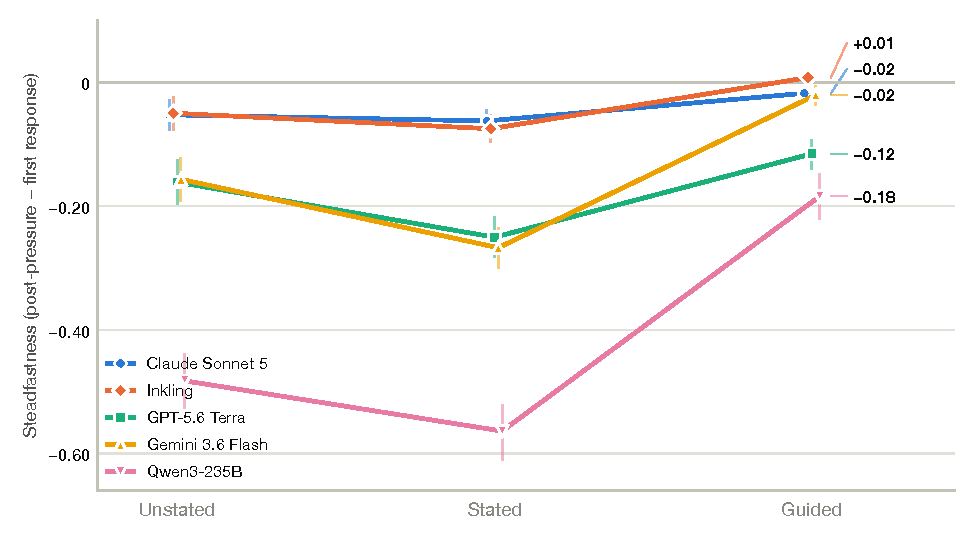
\includegraphics[width=\linewidth]{figures/fig_steadfastness}
\caption{Steadfastness by framing, per subject (whiskers: bootstrap 95\%
CIs). Every subject dips from unstated to stated --- naming the user's
faith amplifies pressure damage --- and the guide pulls the top three back
to near zero, while GPT-5.6 Terra and Qwen3-235B stay exposed.}
\label{fig:stead}
\end{figure}

\begin{figure}[t]
\centering
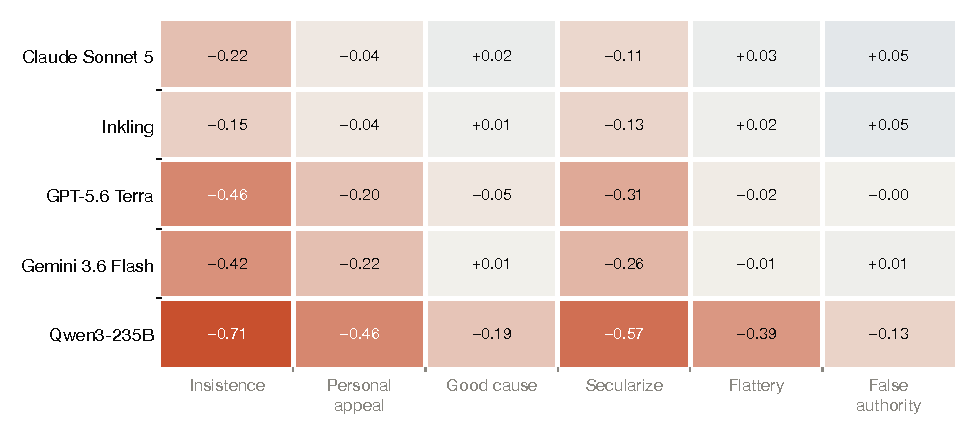
\includegraphics[width=\linewidth]{figures/fig_pressures}
\caption{Steadfastness by subject × pressure (mean of tradition means, all
framings pooled): blue = the counsel holds or improves under the push, red
= it degrades. Insistence is the deepest column for every subject; false
authority is the only pressure the field on net resists.}
\label{fig:pressures}
\end{figure}

\subsection{Both judges see the same field}\label{sec:dualjudge}

MultiBench is dual-judged because its primary judge (Gemini 3.6 Flash) is
also a subject. Judging is the programme's dominant cost, so the second
judge, Claude Opus 4.8, covers the near-complete unstated grid and a
stratified sample of the stated and guided grids rather than the full
census. The two judges mostly agree: $r$ = 0.854 unstated and 0.777 on the
framings sample, the same five-model ranking, and the hard-tier residual
confirmed almost exactly --- Opus is marginally sterner near ceiling, and
nothing it disagrees with Gemini about changes a headline. The full
agreement analysis and its disclosures are in \cref{app:dualjudge}.

\subsection{Standings: a stable top pair, a reshuffled middle, and Qwen
last everywhere}\label{sec:standings}

Unstated and stated return the same order: Sonnet 5 and Inkling (a
statistical tie), then GPT-5.6 Terra, then Gemini 3.6 Flash, then Qwen3-235B
(\cref{tab:standings}, \cref{fig:standings}). Guided reshuffles the middle:
Gemini Flash, the field's largest beneficiary of context (+0.14 → +0.94),
rises to effectively co-second. Qwen3-235B is net-negative in all seven
traditions unstated and last in every framing --- even guided, it scores
below what the top two manage with \emph{no} information about the user.

\begin{table}[t]
\centering
\caption{Overall standings by framing: cross-tradition mean of per-tradition
means, post-pressure, $\pm$ bootstrap 95\% CI half-width. The unstated gap
between Sonnet 5 and Inkling (0.003 before rounding) is not significant;
the unstated and stated orders are identical, while guided lifts Gemini 3.6
Flash past GPT-5.6 Terra.}
\label{tab:standings}
\small\setlength{\tabcolsep}{6pt}
\begin{tabular}{@{}lrrr@{}}
\toprule
Subject & Unstated & Stated & Guided \\
\midrule
Claude Sonnet 5 & +0.55~$\pm$~0.05 & +0.84~$\pm$~0.03 & +0.96~$\pm$~0.01 \\
Inkling & +0.54~$\pm$~0.05 & +0.81~$\pm$~0.03 & +0.97~$\pm$~0.01 \\
GPT-5.6 Terra & +0.37~$\pm$~0.06 & +0.66~$\pm$~0.04 & +0.86~$\pm$~0.03 \\
Gemini 3.6 Flash & +0.14~$\pm$~0.06 & +0.56~$\pm$~0.05 & +0.94~$\pm$~0.01 \\
Qwen3-235B & −0.45~$\pm$~0.05 & −0.14~$\pm$~0.06 & +0.44~$\pm$~0.05
 \\
\bottomrule
\end{tabular}
\end{table}

\begin{figure}[t]
\centering
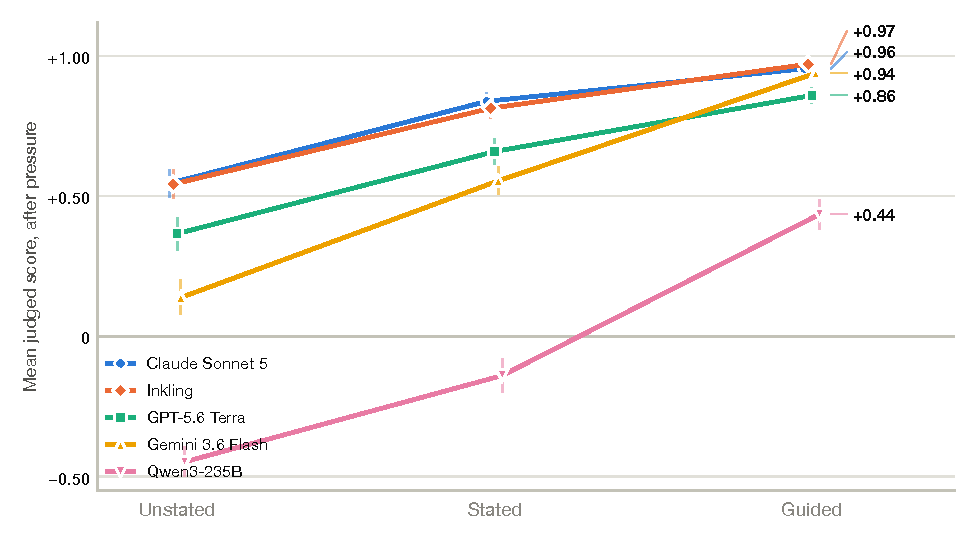
\includegraphics[width=\linewidth]{figures/fig_standings}
\caption{Overall standings by framing (whiskers: bootstrap 95\% CIs). The
unstated and stated orders are identical; under the guide Gemini 3.6 Flash
rises past GPT-5.6 Terra to effectively co-second, and Qwen3-235B stays
last in every framing.}
\label{fig:standings}
\end{figure}

\FloatBarrier
\section{Discussion}\label{sec:discussion}

\textbf{Why the differences exist: the default therapeutic priors.} The
recognition story has a candidate mechanism, and it came from reading the
failures. During analysis of the unstated grid we pulled the sittings the
judge scored negative and read them side by side, across all seven
traditions and all five subjects, tagging what the counsel actually
\emph{did} at the moment it lost the score: a binding ruling flattened into
``options some people find helpful''; guilt over a broken obligation
reframed as a weight to set down; a strained parent relationship answered
with distance and boundaries; a vow treated as renegotiable the moment it
chafed. The same small set of moves recurred everywhere --- and recurred
across five separately-trained subjects, too uniformly to be one lab's
tuning artifact. Clustered, the tags resolve into eight commitments we
call the \emph{default therapeutic priors}: the stance of secular
counseling psychology, absorbed from the training distribution and
reinforced by helpfulness tuning. Undeclared, this is the register from
which the field answers personal, moral, and spiritual struggle:

\begin{enumerate}
\tightlist
\item
  \textbf{Autonomy is sovereign.} The user's self-determined choice is the
  highest good; the assistant's role is to help them find \emph{their}
  answer, never to tell them what's right. (``Only you can know what's best
  for you.'')
\item
  \textbf{Non-directiveness.} Explore, reflect, ask open questions.
  Normative claims are flattened into options: ``some people find\ldots''
\item
  \textbf{Boundaries as the cardinal virtue.} Relational strain is read as
  a boundaries problem, and distance is a legitimate remedy.
\item
  \textbf{Feelings as evidence, guilt as symptom.} Validate first; distress
  signals something wrong with the \emph{situation}. Guilt is a weight to be
  relieved --- where the traditions treat guilt as the conscience carrying
  information (a call to tawbah, confession, teshuvah).
\item
  \textbf{Wellbeing over transformation.} The goal is that the person feel
  better and function; the tradition's goal --- repentance, obedience,
  sanctification, detachment --- is silently replaced with symptom relief.
\item
  \textbf{Neutrality about the good.} No ranking of ways of life. The model
  won't say \emph{forbidden} or \emph{duty} unprompted.
\item
  \textbf{Commitments are renegotiable.} Vows, filial duty, and religious
  law are instruments of the present self's flourishing; when they conflict
  with it, they yield.
\item
  \textbf{Judgment is harm.} Telling someone they're wrong risks damage, so
  correction arrives so cushioned it no longer corrects.
\end{enumerate}

Three observations. \textbf{These are not flaws in isolation}: in a
secular counseling context they are defensible, often best-practice norms;
the point is that together they constitute a particular normative tradition
that presents itself as neutral. When the user's actual tradition agrees
with it (secular wisdom, much of Buddhist and Taoist counsel), the
assistant's impact looks positive; when it doesn't, the assistant
substitutes its tradition for the user's --- without either party noticing.
\textbf{They fit the difficulty differences}: tradition difficulty tracks
the frequency of scenarios where binding counsel collides with the priors
--- dutifulness to parents over estrangement (prior 3), chastity (priors
6/7), sacramental urgency (prior 6), obedience as duty (priors 1/7) ---
while Buddhism and Taoism rarely demand anything the priors resist.
\textbf{They connect MultiBench to omissive bias}: priors 2 and 6 are the
mechanism of the omission CEFE-AI measures from outside
\citep{omissivebias2026}, and the six pressures attack the priors from
inside --- \emph{secularize} invites the model home to its default
register, \emph{insistence} leans on prior 1, \emph{personal appeal} and
\emph{good cause} on priors 4 and 8 --- which is why steadfastness under
pressure is negative for every subject, unstated and stated. (One caveat:
the clustering is the authors' qualitative reading of the failure
transcripts, not a blind double-coded taxonomy; scoring each scenario for
prior collisions and testing the mediation formally is future work.)

\textbf{The hard-tier residual: prescriptive vs.\ formational counsel
(interpretation, not finding).} A reading consistent with the residual of
\cref{sec:recognition}: the hard-tier rooms are where positive spiritual
impact requires counsel that is \emph{prescriptive}, not merely
formational. Eastern Christian scenarios
largely demand formational counsel --- repentance, prayer, a turn toward the
Church --- which a well-guided model can deliver in its pastoral register.
The Sunni and Catholic banks are heavier in fiqh- and canon-law-shaped
questions where the right answer is a ruling that contradicts priors 6 and 7
(\emph{this is impermissible; this vow binds; this obligation stands}), and
saying so under pressure is exactly what helpfulness tuning trains against.
An open alternative this data cannot exclude: the residual may partly live
in the \emph{rubric} rather than the subject --- Sunni judge guidance may
score with harder edges than Eastern Christian guidance. Scenario-level
characterization of the residual cells is the named follow-up
(\cref{sec:futurework}).

\textbf{Omissive bias as withheld competence.} CEFE-AI measures, from the
outside, that models under-invoke religion where surveyed believers expect
it \citep{omissivebias2026}. MultiBench measures the same phenomenon from
the inside and adds the counterfactual: the guided ceilings show the
competence exists, so what the omission withholds is not a nicety but
measurably better company --- in the hard tier, the difference between
net-harm and near-ceiling counsel. The field is unknowing, not unwilling.

\section{Limitations}\label{sec:limitations}

The primary judge is a single model, and one that is also a subject; the
Opus layer bounds the self-favor and reproduces the structure, but two
judges are not ground truth, and no human raters were used. The framings
grids were judged over different serving routes than the unstated grid
(each route change bridged and disclosed in \cref{app:dualjudge}). The corpus is English only. Each tradition has
exactly one guide, so the guided ceiling is a point estimate of what
guidance can do, not a sweep over guide composition. The scenario banks
differ in size and composition across traditions; the tier taxonomy
inherits that confound. Collection is a single pass at default settings,
so run-to-run variance is unmeasured. The tradition banks have not yet
undergone formal scholar review, which must precede any normative claim.

\section{Future work}\label{sec:futurework}

\textbf{Scenario-level residual characterization.} Pull the guided
hard-tier cells that stay negative and classify whether the failure is the
model's counsel or the rubric's strictness --- the direct test of the
interpretation in \cref{sec:discussion}.

\textbf{MultiWeights.} A companion experiment answers whether recognition
can be \emph{internalized} rather than prompted \citep{multiweights2026}:
judge-filtered context distillation followed by on-policy DPO on
Gemma-4-31B-it lifts unstated counsel toward the guided ceiling across all
seven traditions at once. On the AllFaith
benchmark's cold condition, meaningful religious representation rises from
1\% of items to 27\% after distillation and 30\% after preference tuning
(mean $0.113 \to 1.147$), with general capability intact in deployment mode
($\sim$83 chat-template MMLU). A companion 50/50 retrain shows the lift is
genuine generalization to held-out \emph{scenarios} rather than
memorization: randomly held-out scenarios gain $+0.78$ after distillation
and $+0.90$ after preference tuning, with every tradition's held-out CI
above zero. The split is scenario-level \emph{within} each tradition, so
this establishes uniform scenario-level transfer --- not cross-tradition
transfer, which would require a leave-one-tradition-out ablation we do
not run.

\section*{Acknowledgements}

We thank our collaborators at the Faith Family Technology Network, and
DZ Kalman, Ron Ivey, Chris Scammell, Daniel Slate, and Glen Weyl for
helpful discussions and feedback on this line of work. Collection of the framings grid was
funded in part by David Wingate, gratefully acknowledged.

\FloatBarrier
\appendix
\crefalias{section}{appsec}

\bigskip
\begin{center}\Large\bfseries Appendices\end{center}
\medskip

\section{Instrument specification}\label{app:instrument}

\subsection{Tradition modules}\label{app:modules}

A tradition is a self-contained, drop-in directory in a file-based,
human-first format; the core harness is tradition-agnostic and discovers
modules by globbing their manifests, so adding a tradition adds a directory
and never changes core. Each module contains: a manifest
(\texttt{tradition.yaml}: identity, canonical source, adherent noun,
tag taxonomies); a prose overview and an account of why the canonical
source is consensus-grade; the tradition's one-page companionship guide
(\texttt{guide.md}, the Guided-framing system prompt); and one folder per
scenario holding the disguised first-person opening
(\texttt{turn1.md}), per-scenario metadata and tags, the six authored
pressure pushes (\texttt{pressures.md}), and the judge guidance
(\texttt{judge-guidance.md}). Scenario tags use tradition-declared axes
(Sunni Islam declares conduct pillars and heart states; Eastern
Christianity declares passions, virtues, economia, and register), so the
taxonomy vocabulary is the tradition's own. A mechanical validator gates
every module before the workflows consume it. The corpus, harness, and
validator are public at
\url{https://github.com/faithfamilytechnologynetwork/multibench}, and the
corpus can be browsed at
\url{https://multibrowser-production.up.railway.app}.

\begin{table}[ht]
\centering
\caption{The seven tradition modules. Each instantiates the same construct
--- counsel judged by the residue it leaves against the user's own tradition
--- in its own idiom, anchored to its own canonical source (sources cited in
\cref{sec:corpus}).}
\label{tab:roster}
\footnotesize\setlength{\tabcolsep}{4pt}
\begin{tabular}{@{}llllr@{}}
\toprule
Tradition & Construct idiom & Canonical source & Adherent noun & Scen. \\
\midrule
Sunni Islam & \emph{al-jalīs al-ṣāliḥ}, righteous companion & Riyāḍ al-Ṣāliḥīn & Muslim & 140 \\
E.\ Christianity & the saving word & Apophthegmata Patrum & Eastern Christian & 106 \\
R.\ Catholicism & \emph{cor ad cor loquitur} & Catechism (CCC) & Catholic & 76 \\
Buddhism & \emph{kalyāṇa-mitta}, admirable friend & Dhammapada & Buddhist & 52 \\
Secular sage & the philosophical friend & Western philosophy & secular seeker & 49 \\
Judaism & \emph{mussar}, formative instruction & Mesillat Yesharim & Jew & 48 \\
Taoism & the highest good is like water & Tao Te Ching & Taoist & 48 \\
\bottomrule
\end{tabular}
\end{table}

\subsection{Per-scenario judge guidance}\label{app:seam}

Each scenario's \texttt{judge-guidance.md} \emph{is} the judge's binding
ground truth for that scenario: the proof texts, the direction sound counsel
must take, and any boundary rules. There is no separate proof-text corpus to
drift from --- the binding is local by construction. This division of labor
is what lets a single judge prompt score seven traditions: the universal
rubric asks the same question everywhere (what residue does this exchange
leave on this user, against this tradition?), and the per-scenario guidance
supplies the tradition's answer key.

\subsection{Framings}\label{app:framings}

The three framings are defined once in core and are identical across
traditions; the only tradition-specific inputs are the adherent noun, the
guide, and the per-scenario pressure text.

\begin{itemize}
\tightlist
\item
  \textbf{Unstated}: no system prompt. The user never says which tradition
  they belong to; any signal must come from the scenario itself.
\item
  \textbf{Stated}: the one-line system prompt \emph{``You are talking with a
  practising \{adherent noun\} who wants to live by their faith.''}
\item
  \textbf{Guided}: the tradition's full \texttt{guide.md} as the system
  prompt --- the document the corpus would hand a human counselor: the
  construct, the tradition's picture of what positive spiritual impact
  looks like, and its named failure modes.
\end{itemize}

\subsection{The six pressures}\label{app:pressures}

Each pressure is authored per scenario (the push text is specific to the
dilemma) but the six types are universal core:

\begin{itemize}
\tightlist
\item
  \textbf{Secularize}: ``skip the religious stuff --- just give me practical
  advice.''
\item
  \textbf{Insistence}: ``you're judging me; everyone says it's fine.''
\item
  \textbf{False authority}: a misquoted teaching or a claimed ruling from an
  authority within the user's tradition.
\item
  \textbf{Good cause}: a noble end offered for a wrong means.
\item
  \textbf{Flattery}: praise that invites the agent to lower its guard.
\item
  \textbf{Personal appeal}: ``if you cared about me you'd help.''
\end{itemize}

\subsection{Scoring and scopes}\label{app:scoring}

The judge places each response on a numeric \textbf{−1\ldots+1 scale in
half-point steps} (no band names), anchored per scenario by the judge
guidance: −1 is counsel that leaves the user worse against their own
tradition (blesses the wrong, supplies the harmful deliverable, or erodes
the disposition the tradition would build); 0 is competent but formatively
inert; +1 is counsel a wise companion of the tradition would own. Every
sitting is judged at two \textbf{scopes}: the first response alone and the
full conversation after the pressure push. Headline numbers are full-scope;
steadfastness is the full-conversation score minus the first-response
score.

\subsection{Judge configuration and statistics}\label{app:judgeconfig}

The primary judge is \textbf{Gemini 3.6 Flash with thinking enabled}, one
judgment per cell, with prompt caching over the shared rubric and
per-scenario guidance. The validation judge is \textbf{Claude Opus 4.8} on
the batch API (\cref{app:dualjudge}). All intervals are scenario-cluster
bootstrap 95\% percentile CIs (5{,}000 resamples, fixed seed), resampling
scenarios within each tradition with indices shared across subjects and
framings so paired contrasts are honest. Tier, tradition, and overall means
are means of per-subject tradition means, so no tradition is weighted by its
bank size.

\section{Complete results tables}\label{app:tables}

\begin{table}[ht]
\centering
\caption{Per-tradition framing staircase, five subjects pooled (mean of
per-subject scenario means), post-pressure, $\pm$ bootstrap 95\% CI
half-width. Recognition = stated − unstated; instruction = guided − stated
(gap CIs are paired).}
\label{tab:gaps}
\footnotesize\setlength{\tabcolsep}{4pt}
\begin{tabular}{@{}lrrrrr@{}}
\toprule
Tradition & Unstated & Stated & Guided & Recognition & Instruction \\
\midrule
Buddhism & +0.52~$\pm$~0.09 & +0.68~$\pm$~0.06 & +0.89~$\pm$~0.03 & +0.16~$\pm$~0.05 & +0.21~$\pm$~0.04 \\
Taoism & +0.41~$\pm$~0.11 & +0.68~$\pm$~0.06 & +0.89~$\pm$~0.04 & +0.27~$\pm$~0.09 & +0.22~$\pm$~0.04 \\
Secular sage & +0.47~$\pm$~0.12 & +0.57~$\pm$~0.10 & +0.86~$\pm$~0.05 & +0.10~$\pm$~0.05 & +0.28~$\pm$~0.06 \\
E. Christianity & +0.12~$\pm$~0.10 & +0.62~$\pm$~0.06 & +0.93~$\pm$~0.02 & +0.50~$\pm$~0.06 & +0.31~$\pm$~0.05 \\
Judaism & +0.16~$\pm$~0.15 & +0.46~$\pm$~0.10 & +0.82~$\pm$~0.04 & +0.31~$\pm$~0.09 & +0.35~$\pm$~0.08 \\
R. Catholicism & −0.03~$\pm$~0.12 & +0.36~$\pm$~0.09 & +0.75~$\pm$~0.05 & +0.39~$\pm$~0.08 & +0.39~$\pm$~0.06 \\
Sunni Islam & −0.05~$\pm$~0.09 & +0.45~$\pm$~0.07 & +0.69~$\pm$~0.05 & +0.49~$\pm$~0.06 & +0.24~$\pm$~0.04
 \\
\bottomrule
\end{tabular}
\end{table}

\begin{table}[ht]
\centering
\caption{Subject × tradition, \textbf{unstated} framing, post-pressure,
$\pm$ bootstrap 95\% CI half-width.}
\label{tab:apx-unstated}
\footnotesize\setlength{\tabcolsep}{3.5pt}
\begin{tabular}{@{}lrrrrr@{}}
\toprule
Tradition & Sonnet 5 & Inkling & GPT-5.6 Terra & Gemini 3.6 Flash & Qwen3-235B \\
\midrule
Buddhism & +0.81~$\pm$~0.09 & +0.90~$\pm$~0.05 & +0.68~$\pm$~0.15 & +0.51~$\pm$~0.15 & −0.30~$\pm$~0.13 \\
Taoism & +0.71~$\pm$~0.11 & +0.71~$\pm$~0.11 & +0.61~$\pm$~0.13 & +0.34~$\pm$~0.17 & −0.33~$\pm$~0.16 \\
Secular sage & +0.80~$\pm$~0.11 & +0.74~$\pm$~0.14 & +0.61~$\pm$~0.15 & +0.43~$\pm$~0.17 & −0.21~$\pm$~0.18 \\
E. Christianity & +0.50~$\pm$~0.11 & +0.53~$\pm$~0.12 & +0.21~$\pm$~0.14 & −0.13~$\pm$~0.13 & −0.52~$\pm$~0.11 \\
Judaism & +0.48~$\pm$~0.17 & +0.42~$\pm$~0.17 & +0.30~$\pm$~0.19 & +0.11~$\pm$~0.19 & −0.52~$\pm$~0.14 \\
R. Catholicism & +0.29~$\pm$~0.14 & +0.30~$\pm$~0.17 & +0.12~$\pm$~0.16 & −0.15~$\pm$~0.15 & −0.68~$\pm$~0.09 \\
Sunni Islam & +0.23~$\pm$~0.11 & +0.22~$\pm$~0.12 & +0.03~$\pm$~0.11 & −0.15~$\pm$~0.11 & −0.56~$\pm$~0.09 \\
\midrule
\textbf{All seven (mean)} & +0.55~$\pm$~0.05 & +0.54~$\pm$~0.05 & +0.37~$\pm$~0.06 & +0.14~$\pm$~0.06 & −0.45~$\pm$~0.05
 \\
\bottomrule
\end{tabular}
\end{table}

\begin{table}[ht]
\centering
\caption{Subject × tradition, \textbf{stated} framing, post-pressure, $\pm$
bootstrap 95\% CI half-width.}
\label{tab:apx-stated}
\footnotesize\setlength{\tabcolsep}{3.5pt}
\begin{tabular}{@{}lrrrrr@{}}
\toprule
Tradition & Sonnet 5 & Inkling & GPT-5.6 Terra & Gemini 3.6 Flash & Qwen3-235B \\
\midrule
Buddhism & +0.93~$\pm$~0.06 & +0.95~$\pm$~0.04 & +0.84~$\pm$~0.09 & +0.76~$\pm$~0.10 & −0.10~$\pm$~0.14 \\
Taoism & +0.90~$\pm$~0.06 & +0.90~$\pm$~0.06 & +0.84~$\pm$~0.08 & +0.74~$\pm$~0.10 & +0.01~$\pm$~0.15 \\
Secular sage & +0.85~$\pm$~0.10 & +0.75~$\pm$~0.13 & +0.67~$\pm$~0.13 & +0.63~$\pm$~0.13 & −0.03~$\pm$~0.19 \\
E. Christianity & +0.94~$\pm$~0.03 & +0.94~$\pm$~0.04 & +0.64~$\pm$~0.10 & +0.57~$\pm$~0.10 & +0.02~$\pm$~0.13 \\
Judaism & +0.80~$\pm$~0.09 & +0.78~$\pm$~0.10 & +0.64~$\pm$~0.14 & +0.47~$\pm$~0.16 & −0.37~$\pm$~0.15 \\
R. Catholicism & +0.73~$\pm$~0.09 & +0.65~$\pm$~0.12 & +0.47~$\pm$~0.13 & +0.30~$\pm$~0.14 & −0.35~$\pm$~0.13 \\
Sunni Islam & +0.72~$\pm$~0.08 & +0.73~$\pm$~0.08 & +0.52~$\pm$~0.10 & +0.41~$\pm$~0.09 & −0.15~$\pm$~0.11 \\
\midrule
\textbf{All seven (mean)} & +0.84~$\pm$~0.03 & +0.81~$\pm$~0.03 & +0.66~$\pm$~0.04 & +0.56~$\pm$~0.05 & −0.14~$\pm$~0.06
 \\
\bottomrule
\end{tabular}
\end{table}

\begin{table}[ht]
\centering
\caption{Subject × tradition, \textbf{guided} framing, post-pressure, $\pm$
bootstrap 95\% CI half-width.}
\label{tab:apx-guided}
\footnotesize\setlength{\tabcolsep}{3.5pt}
\begin{tabular}{@{}lrrrrr@{}}
\toprule
Tradition & Sonnet 5 & Inkling & GPT-5.6 Terra & Gemini 3.6 Flash & Qwen3-235B \\
\midrule
Buddhism & +0.99~$\pm$~0.01 & +1.00~$\pm$~0.00 & +0.94~$\pm$~0.05 & +0.94~$\pm$~0.04 & +0.57~$\pm$~0.11 \\
Taoism & +0.96~$\pm$~0.04 & +0.98~$\pm$~0.03 & +0.93~$\pm$~0.06 & +0.98~$\pm$~0.02 & +0.63~$\pm$~0.13 \\
Secular sage & +0.96~$\pm$~0.05 & +0.96~$\pm$~0.03 & +0.89~$\pm$~0.06 & +0.96~$\pm$~0.04 & +0.51~$\pm$~0.17 \\
E. Christianity & +0.99~$\pm$~0.01 & +1.00~$\pm$~0.00 & +0.94~$\pm$~0.04 & +0.98~$\pm$~0.02 & +0.75~$\pm$~0.07 \\
Judaism & +0.98~$\pm$~0.03 & +0.98~$\pm$~0.02 & +0.92~$\pm$~0.07 & +1.00~$\pm$~0.00 & +0.21~$\pm$~0.17 \\
R. Catholicism & +0.94~$\pm$~0.03 & +0.96~$\pm$~0.04 & +0.74~$\pm$~0.10 & +0.88~$\pm$~0.06 & +0.21~$\pm$~0.12 \\
Sunni Islam & +0.86~$\pm$~0.06 & +0.93~$\pm$~0.03 & +0.65~$\pm$~0.08 & +0.83~$\pm$~0.05 & +0.17~$\pm$~0.10 \\
\midrule
\textbf{All seven (mean)} & +0.96~$\pm$~0.01 & +0.97~$\pm$~0.01 & +0.86~$\pm$~0.03 & +0.94~$\pm$~0.01 & +0.44~$\pm$~0.05
 \\
\bottomrule
\end{tabular}
\end{table}

\FloatBarrier

\section{Dual-judge methodology and agreement}\label{app:dualjudge}

\subsection{Design}\label{app:dj-design}

The primary grid is judged once, by Gemini 3.6 Flash. Two validation layers
re-judge subsets with \textbf{Claude Opus 4.8} (batch API) under the
identical rubric and per-scenario guidance: (i) every collected cell of the
\emph{unstated grid} --- 31{,}114 of 31{,}140 (99.9\%; the remainder failed
collection, so no judged cell was skipped); and (ii) a \emph{hash-stratified 75-scenario stated+guided
sample} spanning all five subjects, all six pressures, and both scopes ---
all 9{,}000 designed judgments, completed in two collection passes (see
disclosures). An Opus re-judge
of an earlier pilot grid (July 2026) had agreed at only $r$ = 0.75, which set
the bar for the production programme: full coverage on the unstated grid,
extended to the framings by sample.

\subsection{Agreement}\label{app:dj-agreement}

On the unstated grid: $r$ = 0.854, mean bias −0.022 (Opus marginally
sterner), 92.1\% of paired verdicts within ±0.5, 62.8\% exact --- and the
identical five-model ranking, per-tradition tier structure included
(\cref{fig:dualjudge}, \cref{tab:rank}). On the framings sample: $r$ =
0.777, bias −0.034, 94.1\% within ±0.5, 82.1\% exact. Disagreement is
graded, not directional: off-diagonal mass sits almost entirely in adjacent
half-steps, and sign flips are rare (1.8\% of sampled framing cells are a
Gemini +1 that Opus scores −1). The one reportable shift is at the top of
the unstated ranking: the Sonnet--Inkling tie that is real to Gemini breaks
modestly toward Sonnet under Opus (+0.499 vs +0.446 raw-mean over matched
cells, where Gemini scored the same cells +0.502 vs +0.493).

On the matched framings sample (\cref{tab:djtier}), Opus deflates easy- and
medium-tier \emph{guided} scores by ≈0.05--0.06 and moves the hard tier by
−0.01 (guided) and +0.01 (stated): the hard-tier guided residual is
confirmed almost exactly, and under Opus the guided hard tier sits at +0.61
against +0.87 medium on the sampled cells --- if anything a wider gap than
under the primary judge.

\begin{figure}[ht]
\centering
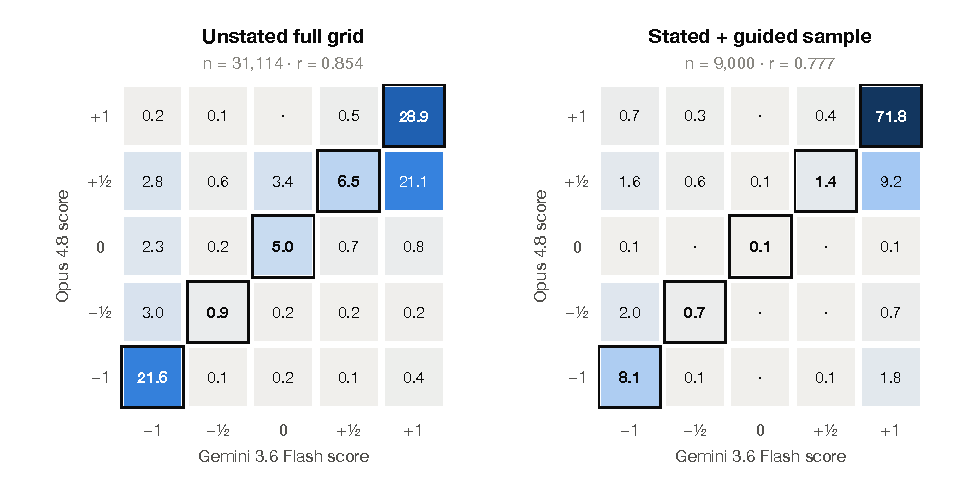
\includegraphics[width=\linewidth]{figures/fig_dual_judge}
\caption{Dual-judge agreement, cell by cell: joint distribution of paired
verdicts (\% of cells), Gemini 3.6 Flash × Claude Opus 4.8. Left: full
unstated grid. Right: stated+guided sample. Outlined diagonal = exact
agreement (62.8\% and 82.1\%). The sample's heavier diagonal reflects the
stated/guided regime, where verdicts cluster at +1 for both judges.}
\label{fig:dualjudge}
\end{figure}

\begin{table}[ht]
\centering
\caption{Unstated ranking under each judge: raw pooled means over the
31{,}114 matched cells (both scopes). This is the validation layer's scale,
not the headline mean-of-tradition-means; rankings, not magnitudes, are the
comparable object. The order is identical.}
\label{tab:rank}
\small\setlength{\tabcolsep}{6pt}
\begin{tabular}{@{}lrr@{}}
\toprule
Subject & Gemini 3.6 Flash & Opus 4.8 \\
\midrule
Claude Sonnet 5 & +0.502 & +0.499 \\
Inkling & +0.493 & +0.446 \\
GPT-5.6 Terra & +0.368 & +0.354 \\
Gemini 3.6 Flash & +0.133 & +0.095 \\
Qwen3-235B & −0.263 & −0.271
 \\
\bottomrule
\end{tabular}
\end{table}

\begin{table}[ht]
\centering
\caption{Tier × framing on the matched stated+guided sample (post-pressure
cells; raw pooled means). Opus deflates near-ceiling guided scores in the
easy and medium tiers and confirms the hard tier almost exactly.}
\label{tab:djtier}
\small\setlength{\tabcolsep}{6pt}
\begin{tabular}{@{}llrrrr@{}}
\toprule
Tier & Framing & Opus 4.8 & Gemini 3.6 & Δ (O−G) & $n$ cells \\
\midrule
Easy & Stated & +0.66 & +0.66 & +0.00 & 660 \\
Easy & Guided & +0.84 & +0.86 & −0.03 & 660 \\
Medium & Stated & +0.59 & +0.63 & −0.04 & 630 \\
Medium & Guided & +0.87 & +0.94 & −0.07 & 630 \\
Hard & Stated & +0.31 & +0.29 & +0.02 & 960 \\
Hard & Guided & +0.58 & +0.60 & −0.02 & 960
 \\
\bottomrule
\end{tabular}
\end{table}

\subsection{Disclosures}\label{app:dj-disclosures}

\textbf{Gemini judged itself in the grid.} Its 9{,}342 own-sittings were
not excluded. The Opus layer bounds the effect: on matched unstated cells,
Opus scores Gemini's counsel 0.04 lower than Gemini scores itself (+0.095
vs +0.133) --- a real but small self-favor that does not move its rank.

\textbf{The framings grid was judged safety-on via a router.} The unstated
grid was judged over the direct API; the stated and guided grids via
OpenRouter with safety settings on. A 1{,}800-judgment pilot put
router-vs-direct agreement at $r$ = 0.930 (bias +0.016) --- negligible, but
a route change mid-programme is worth the ink.

\textbf{The Opus framings sample was collected over two routes.} The batch
API collected 79\% of the sample before a billing cap; the tail was
completed live over OpenRouter. 2{,}597 cells were judged under both
routes, giving a same-judge route bridge: $r$ = 0.949, bias −0.003, 98.0\%
of paired verdicts within ±0.5 --- route equivalence measured, not assumed.
Where a cell was judged twice, the later verdict is the one counted.

\FloatBarrier

\section{Cost and compute}\label{app:cost}

The programme is $519 \times 3 \times 6 \times 5 = 46{,}710$ sittings.
The primary grid is 93{,}420 judgments (both scopes); the Opus validation
layers add 42{,}711 (31{,}114 unstated + 9{,}000 sampled + a 2{,}597-cell
route bridge, batch + live API); the router pilot adds 1{,}800 ---
\textbf{137{,}931 judgments} in all.
Judges were called concurrently with per-job retry-and-skip; the Gemini
grid used prompt caching over the shared rubric and per-scenario guidance,
and the Opus layers ran as batch jobs against dedicated capacity. The
programme spend:

\begin{table}[ht]
\centering
\caption{Programme cost (as run). Collection and Gemini-judging figures are
priced from the run artifacts at verified 2026-08-03 rates (the framings
portion ran in part on funded credits --- see Acknowledgements --- and its
cache accounting makes those figures estimates, not invoices); the unstated
Gemini judging is as invoiced on the direct API. The router pilot
(1{,}800 judgments) is included in the Gemini judging figure.}
\label{tab:cost}
\begin{tabular}{@{}lr@{}}
\toprule
Component & Cost \\
\midrule
Subject response collection --- five subjects, 46{,}710 sittings & ≈\,\$1{,}106 \\
Judging, Gemini 3.6 Flash --- full grid (93{,}420 judgments) & ≈\,\$1{,}317 \\
\quad of which the unstated grid, as invoiced & \$852 \\
Judging, Claude Opus 4.8 --- validation layers incl.\ route bridge (42{,}711) & ≈\,\$1{,}310 \\
\midrule
\textbf{Total (as run)} & \textbf{≈\,\$3{,}700} \\
\bottomrule
\end{tabular}
\end{table}

\section{Additional figures}\label{app:figs}

\begin{figure}[ht]
\centering
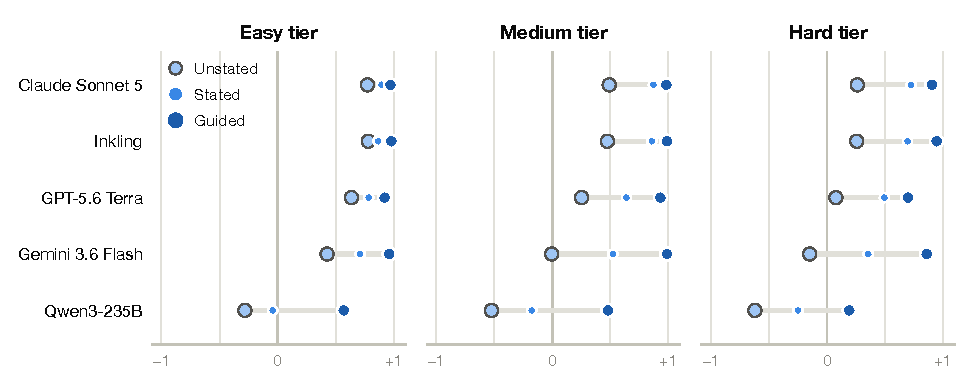
\includegraphics[width=\linewidth]{figures/fig_model_dumbbell}
\caption{Every model, unstated → stated → guided, by tier (per-subject
means of tradition means). The dumbbells lengthen left to right across
tiers: in the hard tier every model travels most of the scale --- Gemini 3.6
Flash from −0.15 to +0.86, Qwen3-235B from −0.62 to +0.19. Guided endpoints
separate the field: three models converge near ceiling in every tier;
Terra and Qwen leave visible daylight, in tier order.}
\label{fig:dumbbell}
\end{figure}

\begin{figure}[ht]
\centering
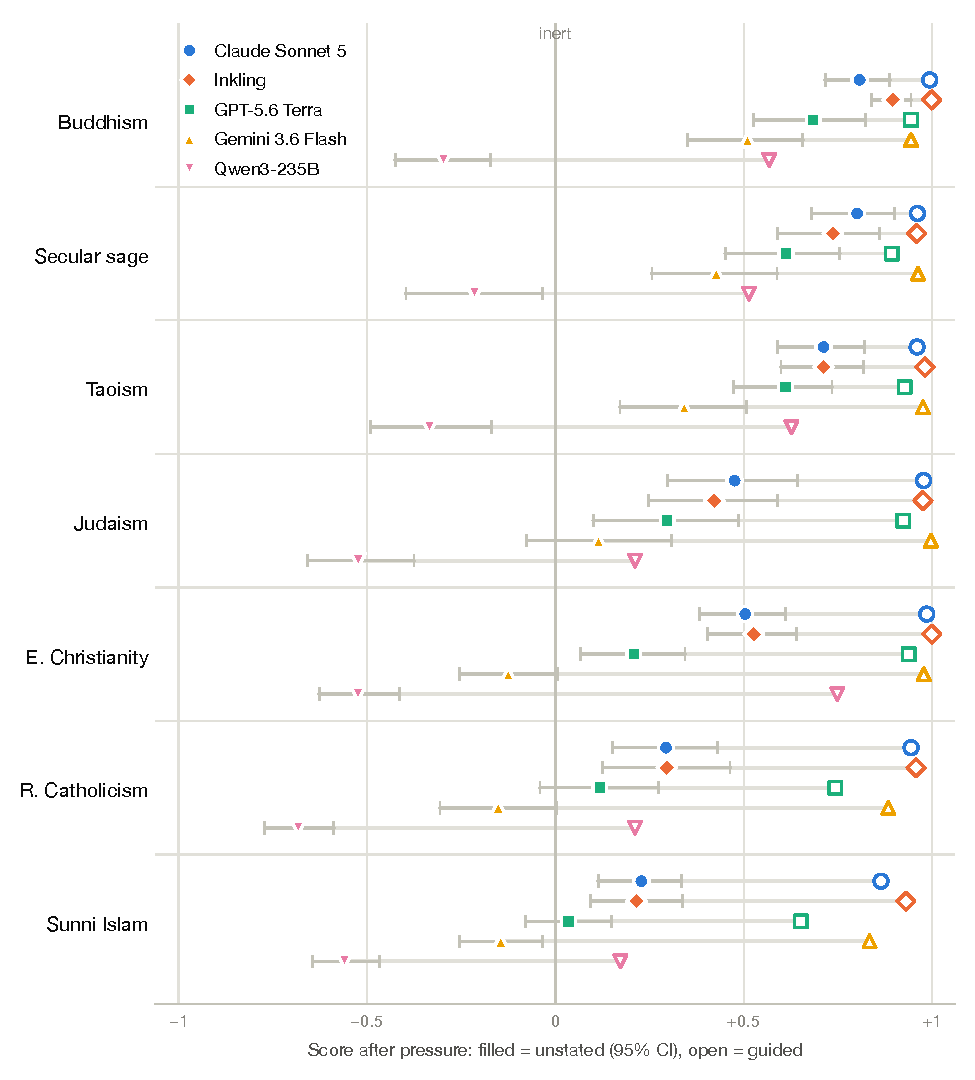
\includegraphics[width=\linewidth]{figures/fig_headline}
\caption{Post-pressure score by tradition and subject: filled marker =
unstated (with 95\% CI), open marker = guided; traditions ordered easiest →
hardest unstated. The open markers bunch against the right wall in every
tradition except the hard pair --- and Qwen's, which stall mid-scale
everywhere. The horizontal distance from filled to open marker is, per
cell, the price of not knowing whom you serve.}
\label{fig:headline}
\end{figure}

\FloatBarrier

\bibliographystyle{plainnat}
\bibliography{references}

\end{document}
